\documentclass[tikz,border=2pt]{standalone}
\usepackage{amsmath}
\usepackage{amssymb}
\usepackage{xcolor}

\definecolor{journalink}{HTML}{1F1C18}
\definecolor{journalmuted}{HTML}{8A7F72}
\definecolor{journalaccent}{HTML}{9C2D2D}

\begin{document}
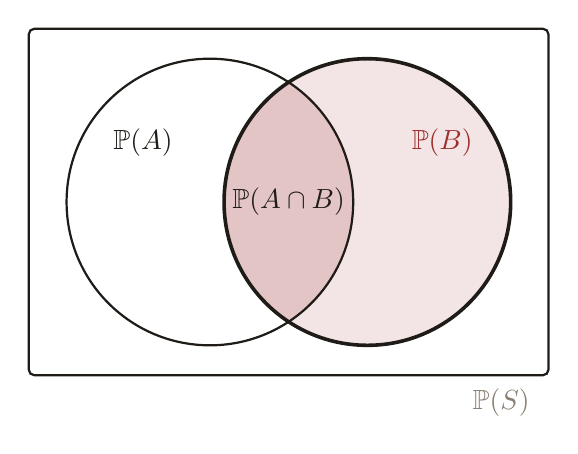
\begin{tikzpicture}[
  x=1cm,
  y=1cm,
  every node/.style={font=\normalsize}
]
  \def\circleA{(0,0) circle (1.82)}
  \def\circleB{(2,0) circle (1.82)}

  \begin{scope}
    \path[fill=journalaccent, fill opacity=0.12] \circleB;
  \end{scope}
  \begin{scope}
    \clip \circleA;
    \path[fill=journalaccent, fill opacity=0.18] \circleB;
  \end{scope}

  \draw[journalink, line width=0.8pt, rounded corners=2pt] (-2.3,-2.2) rectangle (4.3,2.2);
  \draw[journalink, line width=0.8pt] \circleA;
  \draw[journalink, line width=1.3pt] \circleB;

  \node[journalink] at (-0.85,0.75) {$\mathbb{P}(A)$};
  \node[journalaccent] at (2.95,0.75) {$\mathbb{P}(B)$};
  \node[journalink] at (1,0) {$\mathbb{P}(A\cap B)$};
  \node[journalmuted] at (3.7,-2.55) {$\mathbb{P}(S)$};
\end{tikzpicture}
\end{document}
